% Created 2023-05-31 qua 13:30
% Intended LaTeX compiler: pdflatex
\documentclass[11pt]{article}
\usepackage[utf8]{inputenc}
\usepackage[T1]{fontenc}
\usepackage{graphicx}
\usepackage{longtable}
\usepackage{wrapfig}
\usepackage{rotating}
\usepackage[normalem]{ulem}
\usepackage{amsmath}
\usepackage{amssymb}
\usepackage{capt-of}
\usepackage{hyperref}
\usepackage{todonotes}
\usepackage[brazil, portuges]{babel}
\usepackage{amsthm}
\usepackage{setspace}
\doublespacing
\newtheorem{prep}{Preposição}[section]
\usepackage[a4paper, total={6in, 8in}]{geometry}
\usepackage[backend=biber,ittitles,justify,indent,sccite,giveninits,date=year]{biblatex}
\addbibresource{~/arq/bib.bib}
\renewbibmacro{in:}{\ifentrytype{article}{}{\printtext{\bibstring{in}\intitlepunct}}}
\author{Ieremies Vieira da Fonseca Romero}
\date{}
\title{Programação Linear Inteira aplicada a problemas de Coloração em Grafos}
\hypersetup{
 pdfauthor={Ieremies Vieira da Fonseca Romero},
 pdftitle={Programação Linear Inteira aplicada a problemas de Coloração em Grafos},
 pdfkeywords={},
 pdfsubject={},
 pdfcreator={Emacs 28.2 (Org mode 9.6.1)}, 
 pdflang={Portuges}}
\begin{document}

\maketitle
\begin{abstract}
Uma coloração própria de vértices de um grafo consiste em uma alocação de cores tal que nenhum par de vértices adjacentes possuam a mesma cor.
No problema de coloração de vértices, dado um grafo, procuramos uma coloração própria utilizando o menor número possível de cores.
Além de ser um tradicional problema de teoria dos grafos, o problema se apresenta como NP-difícil e resolvê-lo de forma exata é extremamente relevante na atualidade.
Tais aplicações vão desda alocação de recursos como registradores até o gerenciamento de eventos.

Soluções exatas para este problema utilizam técnicas como enumeração com \emph{Branch-and-Bound} \autocite{Furini2016ImprovedDSATURBased}, programação dinâmica \autocites{Eppstein2003SmallMaximalIndependent}[][]{Byskov2002ChromaticNumberTime} ou programação linear inteira.
Nesse projeto, almejamos aplicar a última e utilizar algoritmos de \emph{Branch-and-Price} para superar os resultados da literatura.
Acreditamos que nosso trabalho se diferencia ao aplicar técnicas recentes para tais algoritmos, o que pode levar a uma melhora do estado-da-arte.
Dessa forma, objetivamos resultados competitivos nas instâncias consolidadas na literatura, bem como possíveis novas formulações, cortes e estratégias para melhor resolvê-las.
\end{abstract}

\section{Introdução}
\label{sec:org62a83e2}
Dado um grafo não direcionado, uma \textbf{coloração própria} deste é uma alocação de cores tal que nenhum vértice seja adjacente a outro de mesma cor.
O \textbf{Problema de Coloração de Vértices} (VCP) requer que encontremos uma coloração própria usando o menor número possível de cores.
Decidir se um grafo possui uma coloração própria que usa até \(k \geq 3\) cores é um problema NP-completo \autocite{Garey1979ComputersIntractabilityGuide}, de forma que o problema de otimização também é NP-difícil.

Muitas vezes, deseja-se alocar eventos ou recursos sem que hajam conflitos, seja na divisão de tarefas num cenário de fábricas ou escritórios, ou na organização de eventos.
Assim, desejamos construir uma alocação de eventos a horários sem que, por exemplo, requeira que uma pessoa esteja em dois locais simultaneamente.
Tal problema pode ser convertido a um de coloração transformando cada evento a um vértice no qual dois vértices estão ligados se há necessidade de ao menos uma pessoa estar em ambos eventos.
Assim, numa solução, cada cor irá representar um horário para os eventos acontecerem.

Além dessa, como discutido por \textcite{Malaguti2010surveyvertexcoloring}, diversas são as aplicações do problema, como: agendamento \autocite{Leighton1979GraphColoringAlgorithm}, tabela de horários \autocite{Werra1985introductiontimetabling}, alocação de registradores \autocite{Chow1990prioritybasedcoloring}, comunicação de redes \autocite{Caprara2007PassengerRailwayOptimization} e alocação de banda \autocite{Gamst1986Somelowerbounds}.

As aplicações acima deixam claro que encontrar uma boa (ou até ótima) solução para o problema é crucial.
Cenários reais, muitas vezes, lidam com centenas de milhares de vértices, tornando necessário também resolvermos de forma rápida.

Neste projeto, utilizaremos de Programação Linear Inteira para resolver o problema de forma exata, como discutido na Seção \ref{metodologia}.
É importante mencionar que Programação Dinâmica também é comumente utilizada \autocites{Eppstein2006SmallMaximalIndependent}[][]{Byskov2002ChromaticNumberTime}, mas que vê apenas desenvolvimentos teóricos sem grande aplicabilidade prática no VCP.
Já técnicas de enumeração baseado em \emph{branch-and-bound} \autocite{Brelaz1979Newmethodscolor} possuem resultados práticos melhores que programação dinâmica, mas ainda são superados por técnicas de programação linear inteira.
Por fim, recomendamos as seguintes revisões bibliográficas sobre o problema  \autocites{Malaguti2010surveyvertexcoloring}[][]{Lewis2015GuideGraphColouring}[][]{Husfeldt2015Graphcolouringalgorithms}[][]{Lima2018ExactAlgorithmsGraph}.

\subsection{Modelo matemático}
\label{sec:org94e3d32}
Durante essa proposta, utilizaremos algumas notações que apresentaremos a seguir.

Seja \(G = (V,E)\) um grafo simples não direcionado, denotamos como \(n = |V|\) a quantidade de vértices e \(m = |E|\) a quantidade de arestas.
Dizemos que a vizinhança aberta \(N(v)\) de um vértice~\(v \in V\) no grafo \(G\) é o conjunto de vértices adjacentes a \(v\).
Já a vizinhança fechada \(N[v] = N(v) \cup \{v\}\) é a vizinhança aberta adicionado do vértice \(v\).

Muitas vezes, nos referimos a uma coloração própria apenas como coloração.
Já uma coloração parcial é a atribuição, segundo as mesmas regras, de uma parte dos vértices e, em geral, utilizaremos essa definição para soluções em construção.
O número cromático de~\(G\), chamado de \(\chi(G)\), é a menor quantidade de cores que pode constituir uma coloração do grafo \(G\).
Por fim, usaremos \(H\) como limitante superior ao número cromático.
Uma cor \(h\) é dita válida para o vértice \(v\) se ela não foi atribuída a nenhum vértice da vizinhança aberta de \(v\).

Um conjunto \(S \subseteq V\) é dito independente em \(G\) se, e somente se, não existem arestas em \(E\) que conectem dois elementos de \(S\).
Perceba que o conjunto de vértices coloridos com mesma cor deve ser um conjunto independente.

\subsection{Problemas similares}
\label{sec:orgd26b137}
O problema de \textbf{Multicoloração de Banda} (BMCP) é a combinação de dois problemas: Coloração de Banda e Multicoloração.
No problema de \textbf{Coloração de Banda}, a diferença entre a cor de cada par de vértices adjacentes deve ser, ao menos, a distância entre os dois vértices.
No problema de \textbf{Multicoloração} uma certa quantidade de cores devem ser alocadas a cada vértice, de forma que um par qualquer de vértices adjacentes não possuam uma cor em comum.

Assim, no BMCP, é necessário atribuir, para cada vértice, uma certa quantidade de cores e, para qualquer par de vértices adjacentes, cada combinação dois a dois de cores atribuídas a eles deve ter diferença maior que a distância entre os vértices.
Este problema permite que situações mais complexas que o VCP sejam modeladas, como a alocação de frequência em telecomunicações \autocite{Aardal2007Modelssolutiontechniques}.

Por outro lado, muitas vezes, o recurso que queremos alocar é limitado.
Para refletir isso, podemos colocar um peso em cada vértice e restringir a soma dos pesos dos vértices alocados a cada uma das cores, uma restrição de capacidade.
Este problema é conhecido como VCP Limitado (BVCP) ou \textbf{Problema de Empacotamento com Conflito} \textcite{Connolly1990KnapsackProblemsAlgorithms}.

Tal restrição de capacidade pode ser adicionada à formulação de atribuição (ASS) para modelar o problema de BVCP sem grandes dificuldades.

Por fim, podemos atrelar a cada vértice um peso e definir o custo de uma cor como o maior peso dentre os vértices que ela colore.
Assim, no \textbf{Problema de Coloração com Pesos}, queremos reduzir o custo total das cores.
Esse problema vê aplicações na \emph{Alocação de Máquinas com Compatibilidade de Tarefas} e \emph{Problema de Decomposição de Matriz em Divisão de tempo para Alocação de Tráfico de Múltiplo Acessos} \autocites{Werra1985introductiontimetabling}[][]{Escoffier2006WeightedColoringfurther}[][]{Finke2008Batchprocessinginterval}.

Além das generalizações apresentadas, existem diversas variações desse problema.
A variante de \textbf{soma mínima} pede para encontramos a coloração com a menor soma de valores associados aos vértices \autocite{Jin2016Algorithmsminimumsum}.
Já a \textbf{equitativa,} é o desafio de encontrar uma coloração que distribua as cores de forma onde a diferença entre a cardinalidade da cor atribuída a dois vértices adjacentes seja pequena \autocite{Meyer1973EquitableColoring}.

\section{Metodologia}
\label{sec:org53eabb2}
\label{metodologia}
A seguir, apresentamos as técnicas que almejamos utilizar bem como abordagens já presentes na literatura disponível.

\subsection{Programação Linear Inteira}
\label{sec:org815ba0a}
\textbf{Programação Linear} é uma técnica de otimização a partir da modelagem de \textbf{programas lineares}.
Nestes, definimos uma função objetivo, a qual queremos maximizar ou minimizar com suas variáveis sujeitas a um conjunto de restrições lineares (equações ou inequações lineares) \autocite{Chvatal1983LinearProgramming}. Um programa linear pode ser escrito da seguinte forma:
\begin{alignat*}{4}
& \omit\rlap{minimize \quad \quad $\displaystyle cx$} \\
& \mbox{sujeito a}&& \quad & Ax & \geq b  & \quad &  \\
&                 &&       & x               & \in \mathbb{R}_+ &      &
\end{alignat*}

Para encontrar soluções viáveis com valores ótimos, conhecemos o algoritmo \textbf{simplex} que, apesar de ter complexidade exponencial, no caso médio executa em tempo polinomial~\autocite{Borgwardt1986SimplexMethodAlgorithms}.
Além deste, é importante mencionar os métodos dos pontos interiores \autocite{Karmarkar1984newpolynomialtime} e elipsoide~\autocite{Bland1981FeatureArticleTheEllipsoid} como alternativas ao simplex.

Para alguns problemas, como o de coloração de grafos, não faz sentido falar em soluções fracionárias, afinal, não conseguimos designar ``meia cor'' a um vértice.
Para isso, restringimos as variáveis aos inteiros, fazendo assim um \textbf{Programa Linear Inteiro}. Caso apenas um subconjunto das variáveis possuam a restrição de integralidade, chamamos esse programa de linear misto.

O que a princípio pode parecer uma pequena alteração, torna o problema computacionalmente muito mais complexo.
Para encontramos boas soluções viáveis para esse tipo de programa, algoritmos como o simplex não são o suficiente.
Para isso, utilizamos técnicas como \emph{branch-and-bound}, que consiste em dividir o problema em subproblemas menores e, durante o processo, encontrar limitantes que permitam diminuir o espaço de busca.

Por fim, é interessante nesse momento traçar o paralelo com a \textbf{Combinatória Poliédrica}.
Definimos um \textbf{poliedro} como um subconjunto \(P \subseteq \mathbb{R}^n\) tal que ele possa ser descrito por meio de inequações lineares em tal espaço, similar aos programas lineares apresentados acima.
Caso esse poliedro seja limitado, o chamamos de \textbf{politopo}.
Dizemos que um subconjunto do poliedro definido por uma inequação é uma \textbf{face}.
Se esta não for igual ao poliedro inteiro, dizemos ser própria e, caso também não seja vazia, dizemos ser não-trivial.

A seguir, apresentamos as metodologias e técnicas que nos são relevantes para resolver o problema de forma exata.
Em geral, as instâncias usadas para os resultados de experimentos computacionais são as apresentadas por \textcite{DIMACSGraphColoringInstances}, que foram atualizadas com o passar dos anos.

\subsection{Atribuição}
\label{sec:org397d6d7}
É possível perceber que \(n\) cores são suficientes para colorir um grafo \(G\). Podemos então definir dois conjuntos de variáveis binárias: \(x_{ih}\) se o vértice \(i\) é colorido com a cor \(h\) e \(y_h\) se a cor \(h\) é utilizada. Dessa forma, construímos a seguinte formulação.

\begin{alignat*}{4}
\label{ass}
\mathrm{(ASS)} \quad & \omit\rlap{minimize  $\displaystyle \sum_{i=1}^n y_h$} \\
& \mbox{sujeito a}&& \quad & \sum_{h=1}^n x_{ih}&= 1        & \quad & i \in V \\
&                 &&   & x_{ih} + x_{jh}    & \leq y_h &   & (i,j) \in E, h=1,\dots,n \\
&                 &&   & x_{ih}    & \in \{0,1\} &   & (i,j) \in E, h=1,\dots,n\\
&                 &&   & y_i       & \in \{0,1\} &   & i \in V
\end{alignat*}
Apesar de sua claridade e simplicidade, tal formulação vê pouca aplicação prática sem que apliquemos técnicas mais sofisticadas.

Esse fato se dá por dois motivos:
\begin{enumerate}
\item Muitas soluções são simétricas umas às outras, já que as cores são indistinguíveis. Uma solução que utiliza \(k\) cores possui \(\frac{n!}{(n-k)!}\) permutações de cores do que é, efetivamente, a mesma solução.
\item A relaxação linear do modelo (quando a restrição de integridade é removida) é extremamente fraca. Assim, resolvê-la ainda nos deixa muito distante da solução ótima inteira.
\end{enumerate}

De modo a resolver tais problemas, \textcite{MendezDiaz2006BranchCutAlgorithm} adicionaram a restrição
\[ y_h \geq y_{h+1} \quad h = 1, \dots, n-1 \]
que garante que a cor \(h+1\) só será utilizada se a cor \(h\) já estiver sendo, quebrando várias simetrias.

Eles também acrescentaram diversas famílias de desigualdades válidas ao politopo do novo modelo que são adicionadas ao algoritmo de \emph{Branch-and-Cut} para fortalecer a relaxação linear além de implementar a estratégia de ramificação proposta por \textcite{Brelaz1979Newmethodscolor} com resultados computacionais satisfatórios.

Um algoritmo de \emph{branch-and-bound} consiste em, durante a árvore de \emph{branch-and-bound}, adicionar desigualdades e cortes válidos para diminuir o espaço de busca. Um corte válido é uma inequação que não elimina nenhuma solução inteira viável do modelo.

Já \textcite{MendezDiaz2008CuttingPlaneAlgorithm} apresentam mais duas variações da formulação ASS: uma onde a quantidade de vértices cuja cor \(h+1\) é atribuída não pode ser maior que a quantidade atribuída a cor \(h\) e outro onde conjuntos independentes são ordenados pelo menor índice e apenas a cor \(h\) pode ser atribuída ao \(h-\text{ésimo}\) conjunto.

\subsection{Representantes}
\label{sec:orga936655}
\textcite{Campelo2004CliquesHolesVertex} propuseram uma formulação baseada em representantes, em que cada cor é representada por um vértice.
Para tal, utilizam a variável binária \(x_{vu}\), para todo \(u, v \in V\) não adjacentes, a fim de representar se o vértice \(v\) é representante da cor de~\(u\) e \(x_{vv}\) se \(v\) é o próprio representante de sua cor.
Seja \(\bar{N}(v)\) o conjunto de vértices não adjacentes de \(v\), esta formulação pode ser escrita como
\begin{alignat*}{4}
\mathrm{(REP)} \quad & \omit\rlap{minimize  $\displaystyle \sum_{v \in V} x_{vv}$} \\
& \mbox{sujeito a}&& \quad & \sum_{u \in \bar{N}(v) \cup \{v\}} x_{uv}&= 1        & \quad & v \in V \\
&                 &&   & x_{vu} + x_{vw}    & \leq x_{vv} &   & v \in V, \forall e = (u,w) \in G[\bar{N}(v)] \\
&                 &&   & x_{vu}       & \in \{0,1\} &   & \forall \text{ $u$ e $v$ não adjacentes ou $v = u$}
\end{alignat*}
O primeiro conjunto de restrições garante que todo vértice terá exatamente um representante enquanto o segundo garante que dois vértices adjacentes terão representantes diferentes.

Como \textcite{Campelo2008AsymmetricRepresentativesFormulation} discutem, existem diversas soluções simétricas para tal modelo que apenas distinguem no representante das cores sem alterar efetivamente a solução.
Eles propõem acrescentar uma ordenação para que apenas o menor vértice possa ser o representante, porém esta versão possui um número exponencial de variáveis e, portanto, requer técnicas como \emph{branch-and-price}, abordada mais afundo na Seção \ref{conjuntos_independentes}.
Os autores também apresentam diversas restrições válidas a fim de reforçar o modelo.

Experimentos computacionais foram feitos por \textcite{Jabrayilov2018NewIntegerLinear} mostrando a capacidade deste modelo de competir com as demais formulações.

\subsection{Conjuntos independentes}
\label{sec:org561f43e}
\label{conjuntos_independentes}
Proposto por \textcite{Mehrotra1996ColumnGenerationApproach}, outra forma de entender o problema é imaginá-lo como um \textbf{problema de cobertura de conjuntos} (SC) onde os conjuntos disponíveis são os conjuntos independentes dos vértices.

Assim, seja \(S\) a família de conjuntos impendentes do grafo \(G\), a variável binária \(x_s\) representa se o conjunto \(s \in S\) está sendo usado ou não na solução. Nossa formulação então se dá por:
\begin{alignat}{4}
\mathrm{(SC)} \quad & \omit\rlap{minimize  $\displaystyle \sum_{s \in S} x_s$} \nonumber \\
& \mbox{sujeito a}&& \quad & \sum_{s \in S: i \in s} x_{s}&\geq 1 & \quad & i \in V \label{rest9} \\
&                 &&   & x_s       & \in \{0,1\} &    & s \in S \nonumber
\end{alignat}
O primeiro conjunto de restrições garante que todos os vértices de \(V\) estão contidos em algum conjunto independente escolhido.
Apesar de poucas restrições, essa formulação sofre de ter um número exponencial de variáveis, o que a torna impraticável de implementá-la em resolvedores convencionais como \emph{Gurobi}.

Por tal motivo, \textcite{Mehrotra1996ColumnGenerationApproach} propuseram um algoritmo de \emph{branch-and-price} baseado nesta modelagem.
Essa abordagem permite lidar com um número exponencial de variáveis, já que iniciamos com um subconjunto destas e adicionamos com o passar do desenvolvimento da árvore de \emph{branch-and-bound}.

Neste algoritmo, a decisão de qual variável será adicionada é feita pelo subproblema de geração de coluna caracteriza um \textbf{Problema de Conjunto Independente de Peso Máximo}:
\begin{alignat*}{4}
& \omit\rlap{maximize  $\displaystyle \sum_{i \in V} \pi_i z_i$} \\
& \mbox{sujeito a}&& \quad & z_i + z_j &\leq 1 & \quad & (i,j) \in E \\
&                 &&   & z_i       & \in \{0,1\} &    & i \in V
\end{alignat*}
onde \(z_i\) é uma variável binária que indica se o vértice \(i\) está incluso no conjunto independente e \(\pi_i\) é o valor ótimo da variável dual associado à restrição \eqref{rest9}.
Tal problema pode ser resolvido de forma heurística para encontrar a coluna de custo reduzido com valor negativo.
Em caso de soluções fracionárias, os autores sugerem uma estratégia que garante que os subproblemas continuam a ser de coloração de vértices e apenas requer que o grafo original seja alterado.

Além disso, \textcite{Malaguti2011ExactApproachVertex} propõem meta-heurísticas para inicialização e geração de colunas bem como novos esquemas de ramificação.

Similar a este último modelo, \textcite{Hansen2009Setcoveringpacking} propuseram a formulação chamada de \textbf{Empacotamento de conjunto} (SP)
\begin{alignat*}{4}
\mathrm{(SP)} \quad & \omit\rlap{minimize  $\displaystyle \sum_{s \in \Omega} (|s| - 1)x_s$} \\
& \mbox{sujeito a}&& \quad & \sum_{s \in \Omega: i \in s} x_{s}&\leq 1 & \quad & i \in V \\
&                 &&   & y_s       & \in \{0,1\} &    & s \in \Omega
\end{alignat*}
em que \(\Omega\) é a família de conjuntos independentes com mais de um elemento.
Para essa formulação, seja \(z\) o valor da solução, a quantidade de cores usadas é igual \(k = n - z\).
Além disso, \textcite{Hansen2009Setcoveringpacking} demonstram a equivalência das formulações de SC e SP, bem como apresentam diversas famílias de inequalidades válidas que definem facetas.
Uma \textbf{faceta} pode ser definida como uma face própria maximal, ou seja, uma face própria que não está contida em nenhuma outra.

Os autores também apresentam resultados computacionais que não demonstram superioridade entre o trabalho deles em relação à \textcite{Mehrotra1996ColumnGenerationApproach} bem como técnicas de pré-processamento e um algoritmo de planos-de-corte.
Um algoritmo de \textbf{planos-de-corte} é aquele que parte de um modelo relaxado, resolve-se e iterativamente acrescenta-se inequações válidas, chamadas de planos-de-corte, para eliminar tal solução.
Repetimos o processo até encontrar uma solução para o problema original.

Já \textcite{Morrison2014WideBranchingStrategy} apresentam outra forma de realizar a ramificação do processo de \emph{branch-and-bound}.
Tradicionalmente, esta é feita dividindo apenas em dois subproblemas, mas os autores propõem uma abrangente quantidade de subproblemas a cada ramificação com intuito de impedir que cheguemos a subgrafos onde o problema de precificação é mais difícil.
Mais uma vez, resultados computacionais provam que a ideia é competitiva com as anteriores.

Recentemente, \textcite{Morrison2016SolvingPricingProblem} propuseram uma estratégia utilizando diagramas de decisão para agilizar a resolução do problema de precificação que, segundo seus experimentos, possui bons resultados práticos bem como fornece limites inferiores durante o processo.

\subsection{Ordenação parcial hibrida}
\label{sec:orgf118477}
Apresentado inicialmente por \textcite{Jabrayilov2018NewIntegerLinear}, essa formulação utiliza um misto do modelo de atribuição e a ordenação parcial.
Para isto, definimos uma ordenação parcial da união do conjunto de vértices e do conjunto ordenado de cores \((1, \dots, H)\) e, portanto, determinamos a ordem relativa de cada vértice com respeito a cada cor.
Dizemos que o vértice \(v\) é colorido com a cor \(h\) se \(h-1 \succ v\) e \(h \nsucc v\) (no caso de \(h=1\), se \(h \nsucc v\)).

Além disso, nesse modelo, é escolhido um vértice arbitrário \(q\) e \(H\) é um limitante superior do número cromático.
A formulação segue:
\begin{alignat*}
\mathrm { (POPH) } \quad & \omit\rlap{minimize  $\displaystyle 1+\sum_{1 \leq h \leq H} g_{h, q}$} \\
& \mbox { sujeito a } && \quad & g_{H, v} &=0          & \quad & \forall v \in V \\
&                     &&   & x_{v, 1} &=1-g_{1, v} & \quad & \forall v \in V \\
&                     &&   & x_{v, h} &=g_{h-1, v}-g_{h, v} & \quad & \forall v \in V, h=2, \ldots, H \\
&                     &&   & x_{u, 1}+x_{v, 1} &\leq g_{1, q} & \quad & \forall u v \in E \\
&                     &&   & x_{u, h}+x_{v, h} &\leq g_{h-1, q} & \quad & \forall u v \in E, h=2, \ldots, H \\
&                     &&   & g_{h, q}-g_{h, v} &\geq 0 & \quad & \forall v \in V, h=1, \ldots, H \\
&                     &&   & g_{h+1, q}-g_{h, v} &\geq 0 & \quad & \forall v \in N(q), h=1, \ldots, H-1 \\
&                     &&   & x_{v, h}, g_{h, v} &\in\{0,1\} & \quad & \forall v \in V, h=1, \ldots, H \text {. } \\
&                     &&   &
\end{alignat*}
O primeiro conjunto de restrições garante que nenhum vértice é maior que a cor H.
Já o segundo e terceiro correlacionam as variáveis de ordenação parcial com as de atribuição, enquanto o quarto e quinto garantem que dois vértices adjacentes não são coloridos com a mesma cor.
Por fim o sexto, força que \(q\) seja o vértice com a maior cor que, juntamente com o sétimo, são utilizados para reforçar a formulação.

\subsection{Diagrama de decisões binárias ordenadas}
\label{sec:orgc21c95b}
Por fim, mais recentemente, \textcite{Hoeve2021Graphcoloringdecision} aplica técnicas de diagrama de decisão.
Nesta, representamos cada atribuição por um arco que liga o ``estado da solução'' antes e depois de tomá-la.
Mais formalmente, para um problema \(P\) definido por um conjunto de variáveis ordenadas \(X = \{x_1,x_2,\dots ,x_n\}\), construímos um diagrama de decisão, um grafo simples acíclico de \(n+1\) níveis.
O primeiro destes, possui apenas um vértice, \(r\), chamado raiz, assim como o último com o vértice \(t\).
O nível \(i\) é um conjunto de nós associados à variável \(x_i\) onde cada um destes possuem arcos para vértices do nível \(i+1\) e tais arcos possuem etiquetas, \(0\) ou \(1\), correspondendo da variável associada.

\textcite{Hoeve2021Graphcoloringdecision} utiliza a formulação de conjuntos independentes para aplicar tal técnica, onde cada variável indica o uso, ou não, de um vértice em um conjunto.
Se conseguíssemos achar um diagrama de decisão que correspondesse exatamente ao problema de coloração, poderíamos resolver o problema por meio de uma formulação de fluxo, na qual cada \(\{r,t\}-\text{caminho}\) seria um conjunto independente e, como demostrado pelos autores, a função objetivo seria nosso número cromático.
Infelizmente, tal diagrama pode conter um número exponencial de nós, requerendo técnicas mais sofisticadas.
Além disso, quando a solução não é exata, a qualidade da solução depende da ordenação das variáveis.

Por exemplo, observe a Figura \ref{fig:diagrama_decisao}.
Ao lado esquerdo está descrito um grafo e ao lado direito, um correspondente diagrama de decisão.
Neste, os números dentro dos nós representam o conjunto de vértices disponíveis, ou seja, o estado, enquanto os arcos tracejados correspondem aos 0-arcos e os contínuos, os 1-arcos.

\begin{figure}[htbp]
\centering
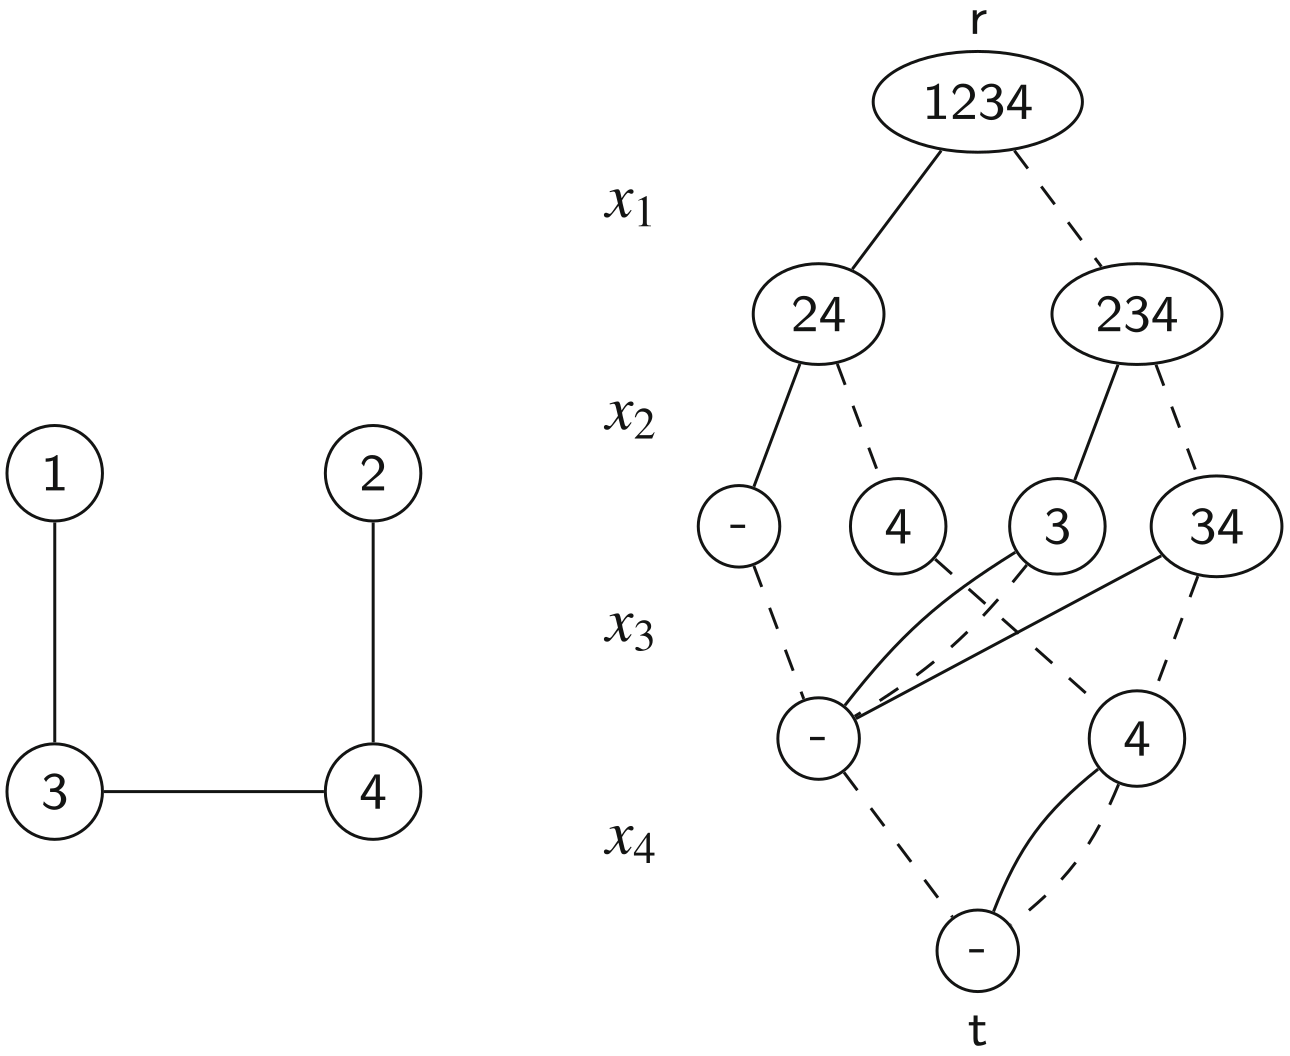
\includegraphics[width=250px]{./diagrama_decisao.png}
\caption{\label{fig:diagrama_decisao}Imagem original por \textcite{Hoeve2021Graphcoloringdecision}. Ao lado esquerdo, um grafo, e ao lado direito, um correspondente diagrama de decisão.}
\end{figure}

Os autores relatam ter obtido resultados competitivos com outros estados-da-arte utilizando estratégias específicas da literatura de diagrama de decisões para resolver as dificuldades apresentadas acima.

\section{Objetivos}
\label{sec:org64da7e3}
Recentemente, houve avanços significativos na abordagem de branch-and-price para o problema de coloração, resultando em vários trabalhos publicados para outros problemas que utilizam e melhoram essa técnica. Um exemplo notável é o trabalho de \textcite{Lima2022Exactsolutionnetwork}, que apresenta técnicas fortes que melhoram o estado da arte para problemas como o Problema de Empacotamento.

Os autores propõem um modelo baseado em fluxo de arcos para auxiliar em algoritmos de geração de colunas.
Eles também comentam que qualquer problema de cobertura de conjunto consegue ser transformado em um problema de fluxo, o que indica que suas técnicas podem ser relevantes para o nosso problema.
Além disso, eles utilizam \textbf{fixação de variáveis}, técnica na qual é possível provar que algumas variáveis nunca poderão entrar no modelo de \emph{branch-and-pricing} e tornar a solução melhor.
A dificuldade reside em encontrar uma solução dual viável que possibilite computar o custo reduzido, necessário para provar esta afirmação.
Um importante desenvolvimento proposto pelos autores é justamente um modelo linear capaz de encontrar eficientemente uma solução, mesmo que não seja ótima (o que, como argumentado por eles, é ainda mais eficiente).

Outro bom indicador do que pretendemos fazer é a semelhança de bons resultados recentes como \textcite{Hoeve2021Graphcoloringdecision} que utilizam ideias muito similares.

Técnicas interessantes também foram propostas por \textcite{Pessoa2021SolvingBinPacking} que apresentam um modelo genérico para resolver problema de roteamento.
Quando se adiciona um corte no \emph{branch-cut-and-price}, isso corresponde a variáveis no dual dificultando o subproblema de geração de colunas.
Os autores utilizam cortes de rank-\(1\) com memória limitada para melhorar tal processo.
Além disso, eles usam \textbf{propagação de etiquetas}, técnica comum na resolução de problemas de precificação que pode ser interessante para o nosso problema.

Nosso principal objetivo é aplicarmos tais novas tecnologias ao problema de coloração.
Além disso, estudaremos a possibilidade de novos cortes e limitantes para as formulações.
Por fim, como apresentado no começo desse projeto, diversos são os problemas similares ou generalizações bem como as aplicações de tais.
Assim, podemos também voltar nossas técnicas e implementações a tais variantes.


\section{Cronograma}
\label{sec:orgf3cd476}
O projeto está dividido em etapas distintas, cada uma com um objetivo específico.
A primeira fase é de revisão bibliográfica, onde serão dedicados \(2\) trimestres para estudar a literatura existente sobre o assunto.
Reforçamos que, apesar deste ser o foco da primeira etapa, a revisão da bibliografia será permanente.
Em seguida, serão dedicados \(2\) trimestres para implementar o estado da arte, onde aplicaremos os conhecimentos adquiridos na fase anterior.
A próxima etapa é o desenvolvimento de novos algoritmos, bem como a implementação e experimentação de tais soluções, onde serão dedicados os trimestres seguintes.
Por último, nos dedicaremos a escrever o relatório final, que apresentará as conclusões e resultados do projeto.

Além disso, é importante notar que é de interesse do aluno realizar um intercâmbio com pesquisadores do exterior, como Manuel Iori.
Pesquisadores como ele possuem vasta experiência tanto no problema quanto na técnica que estudamos e acreditamos que será engrandecedor para o processo de formação do aluno.
Pretendemos concretizar tal intercâmbio no primeiro semestre de \(2024\).

Por fim, o aluno irá, como requerido pela instituição, cursar as três matérias de pós-graduação restantes no primeiro ano, defender seu exame de qualificação de mestrado (EQM) na metade de 2023 e realizar o Programa de Estágio em Docência (PED) no segundo semestre de 2023.

Refletimos o cronograma planejado na Tabela \ref{tab:cron}.

\begin{table}[htbp]
\caption{\label{tab:cron}Cronograma trimestral para este projeto de mestrado, iniciando em Março de 2023.}
\centering
\begin{tabular}{lllllllll}
Atividade & Mar & Jun & Set & Dez & Mar & Jun & Set & Dez\\[0pt]
\hline
Disciplinas & \(\bullet\) & \(\bullet\) &  &  &  &  &  & \\[0pt]
EQM &  & \(\bullet\) &  &  &  &  &  & \\[0pt]
PED &  &  & \(\bullet\) &  &  &  &  & \\[0pt]
Revi. Biblio. & \(\bullet\) & \(\bullet\) & \(\bullet\) &  &  &  &  & \\[0pt]
Implem. estado-da-arte &  &  & \(\bullet\) & \(\bullet\) &  &  &  & \\[0pt]
Desenvolvimento &  &  & \(\bullet\) & \(\bullet\) & \(\bullet\) & \(\bullet\) & \(\bullet\) & \(\bullet\)\\[0pt]
Escrita &  &  &  &  &  &  & \(\bullet\) & \(\bullet\)\\[0pt]
\end{tabular}
\end{table}
Acrescido a isso, o beneficiário deste projeto ministra aulas de Introdução à Programação para alunos de ensino médio na modalidade de itinerários formativos desde \(2022\) em colégio particular de Campinas, SP.
Para o ano de \(2023\), estão programadas \(3\) aulas semanais, o que se mantém consoante a Portaria PR n° \(05/2012\).
Acreditamos que tal atividade muito acrescentará no desenvolvimento do aluno como acadêmico, transmitindo os conhecimentos adquiridos à comunidade e ajudando na divulgação científica.

\section{Material e método}
\label{sec:org8f789be}
Para o desenvolvimento do projeto, o aluno utilizar-se-á de artigos e materiais de consulta disponibilizados pela UNICAMP de maneira gratuita, grande parte desses de forma online ou por meio da Biblioteca do Instituto de Matemática, Estatística e Computação Científica.

Ademais, serão realizados encontros semanais entre o aluno e o orientador para debater os conteúdos estudados e acompanhar o progresso do projeto.

\section{Avaliação dos resultados}
\label{sec:org4a387b1}
Os algoritmos e modelos propostos serão comparados com as instâncias presentes na literatura, como as instâncias do \textcite{DIMACSGraphColoringInstances} e, caso necessário, novas instâncias poderão ser geradas.

Os resultados dos experimentos computacionais serão comparados utilizando técnicas como \textbf{Performance Profile} apresentado por \textcite{Dolan2002Benchmarkingoptimizationsoftware}.

Além disso, pretendemos utilizar técnicas de análise estatística como apresentadas por \textcite{Derrac2011practicaltutorialuse} a fim de produzir comparações mais rigorosas entre as propostas desse projeto.

Por fim, como previsto, serão elaborados relatórios com os resultados obtidos bem como qualquer artigo que seja relevante.

\printbibliography
\end{document}